\documentclass{ohm_project_description}

\projecttitle{Markerlose Indoor-Lokalisierung einer Drohne ohne GNSS}
\projectauthor{Labor für mobile Robotik}
\projectdate{2026}

\begin{document}

\maketitle
\thispagestyle{fancy}

\vspace*{-2.5cm}
\begin{figure}[h!]
    \centering
    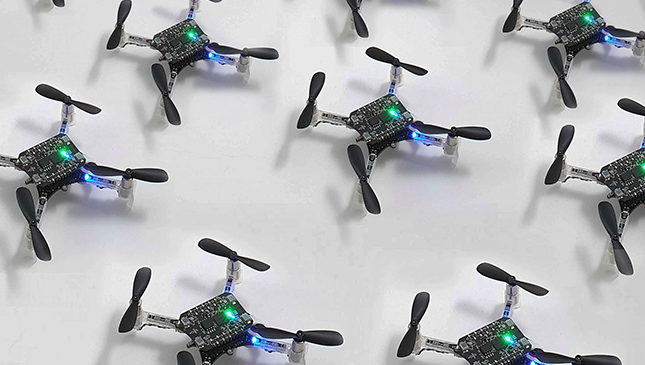
\includegraphics[height=4cm]{img/crazyflies.png}
\end{figure}

Die im AerodrOHM eingesetzte Drohne bestimmt ihre Position bisher über ein externes, markerbasiertes Trackingsystem. Dieses liefert zwar sehr genaue Posen, setzt aber einen fest installierten, instrumentierten Flugraum voraus und ist außerhalb dieses Raums nicht verfügbar. Ziel dieser Arbeit ist es, die bestehende Drohne in die Lage zu versetzen, sich im Innenraum ohne GNSS und ohne Marker allein anhand ihrer Onboard-Sensorik selbst zu lokalisieren.

Die Arbeit baut unmittelbar auf der vorhandenen Drohne und der bestehenden ROS-basierten Systemarchitektur auf. Geeignete Onboard-Sensorik (Kamera, IMU, optional Optical-Flow- oder Tiefensensor) wird integriert und ein markerloses Lokalisierungsverfahren umgesetzt, beispielsweise eine Visual-Inertial Odometry (VIO) oder ein Visual-SLAM-Ansatz. Als Referenz (Ground Truth) für die Evaluation dient das vorhandene markerbasierte Trackingsystem im AerodrOHM.

\section*{Arbeitspakete}
\begin{itemize}[leftmargin=0.5cm]
    \setlength\itemsep{.1em}
    \item Einarbeitung in die bestehende Drohnen-Plattform und das markerbasierte Trackingsystem im AerodrOHM
    \item Auswahl und Integration geeigneter Onboard-Sensorik (Kamera, IMU, ggf. Optical-Flow- oder Tiefensensor)
    \item Implementierung eines markerlosen, GNSS-freien Lokalisierungsverfahrens (z.\,B. Visual-Inertial Odometry oder Visual SLAM)
    \item Integration in die bestehende ROS-Systemarchitektur und Flugregelung
    \item Evaluation der Genauigkeit und Robustheit gegen das markerbasierte Tracking als Ground Truth
    \item Flugversuche und Dokumentation der Ergebnisse im AerodrOHM
\end{itemize}

\section*{Voraussetzungen}
\begin{itemize}[leftmargin=0.5cm]
    \setlength\itemsep{.1em}
    \item Kenntnisse in Programmierung (Python und/oder C++)
    \item Idealerweise erste Erfahrungen mit ROS / ROS 2
    \item Grundkenntnisse in Computer Vision und/oder Zustandsschätzung (z.\,B. Kalman-Filter)
    \item Interesse an Drohnen, Sensorintegration und Lokalisierung
    \item Selbstständige und sorgfältige Arbeitsweise
\end{itemize}

\vspace{0.5cm}
Das Thema kann nach Abstimmung als \textbf{Projekt- oder Bachelorarbeit} bearbeitet werden.

\vfill
\textcolor{ohm_red}{\rule{\linewidth}{0.4mm}}
\textbf{\textcolor{ohm_red}{Labor für mobile Robotik}} \\
\begin{tabular}{@{}ll}
\textbf{Betreuer:} & Prof. Dr. Christian Pfitzner \\
\textbf{E-Mail:}   & \href{mailto:christian.pfitzner@th-nuernberg.de}{christian.pfitzner@th-nuernberg.de} \\
\end{tabular}

\end{document}
